\documentclass[compress]{beamer}

\usepackage{graphicx}

\usetheme{Marburg}

\title{Grafana \& Prometheus}
\author{Parham Houshmand}
\institute{Carriot Inc.}
\date{\today}

\begin{document}

\frame{\titlepage}

\begin{frame}{Overview}

\tableofcontents

\end{frame}

%%%%%%%Section%%%%%%%

\section{What is metrics?}

\begin{frame}

\frametitle{Metrics}

\begin{figure}
\centering
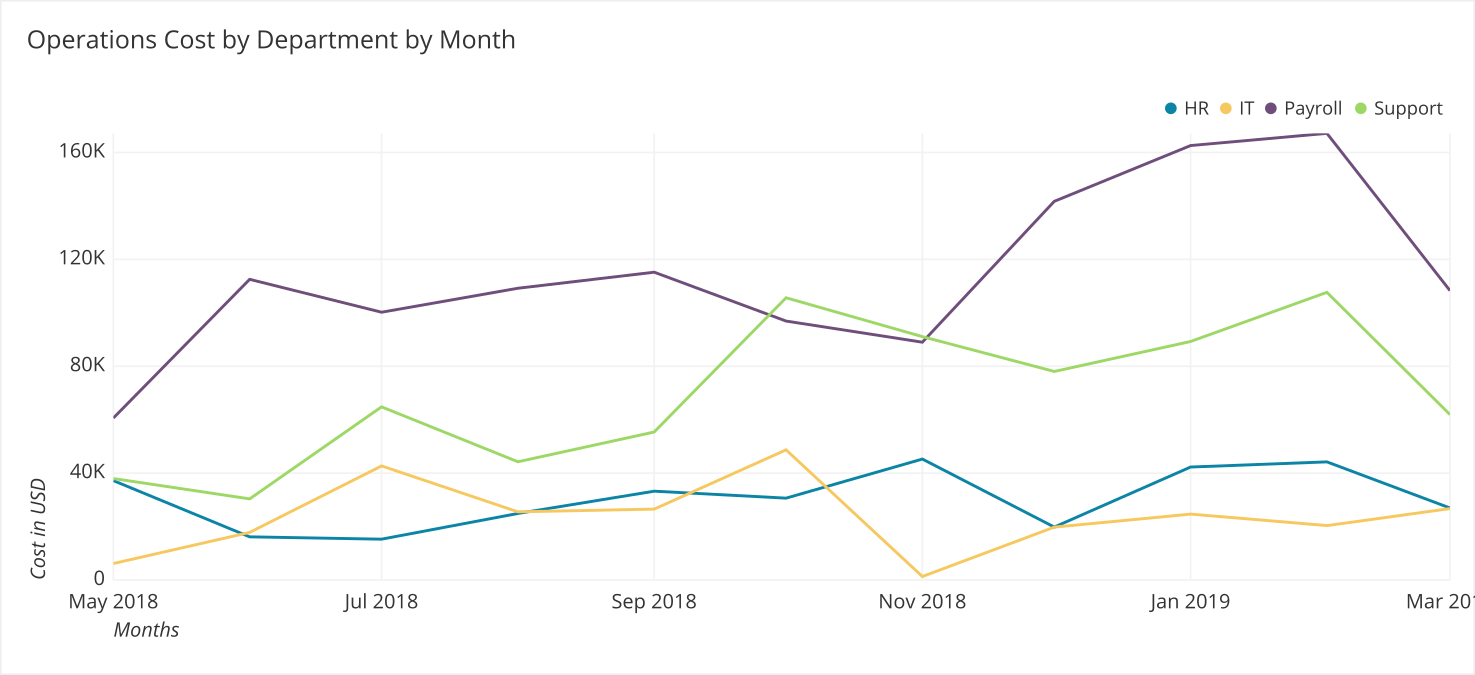
\includegraphics[height=70px]{./images/operationChart.png}
\end{figure}

Metrics represent the raw measurements of resource usage or behavior that can be observed and collected throughout your systems.

\begin{itemize}
\item Monitor performance and reacting to issues or changes in real-time
\item Hostorical trends, track changes in your performance, storage, or error rates
\end{itemize}

\end{frame}

%%%%%%%%%%%%%%%%%%%%

\subsection{Metrics vs Logs vs Traces}
\begin{frame}

\frametitle{Metrics vs Logs vs Traces}

\begin{itemize}

\item \textbf{Metrics} are the numeric representation like percentiles or the averages which helps in monitoring the fate of a system holistically and are measured over an interval of time.

\item \textbf{Log} is an idempotent record of a discrete event that happened in a system at any point of time during the request life cycle. A log usually includes the timestamp and context payload for an event and can be emitted in various forms like plain text, structured format like json or binary logs.

\item \textbf{Tracing} gives the capability to monitor the fate of a request during its lifecycle across various components in a system.
\end{itemize}
\end{frame}

%%%%%%%%%%%%%%%%%%%%

\begin{frame}

\frametitle{Metrics vs Logs vs Traces}

\begin{figure}
\centering

\includegraphics[height=150px]{./images/01.png}
\caption{Relation between metric, log and trace}
\end{figure}

\end{frame}

%%%%%%%%%%%%%%%%%%%%
\subsection{Why using metrics?}
\begin{frame}
\frametitle{Why using metrics?}
\begin{itemize}
\item \textbf{Understand historical trends}

Being able to see and react to how your system is changing is important for maintaining overall health.
\item \textbf{Efficient storage}

Because  metrics give you an aggregated view, they're a really efficient way to store information.

\item \textbf{Faster troubleeshooting}

Many incidents begin with an unexpected change in a metric so metrics are generally your first place to start investing when you identify a problem.
\end{itemize}
\end{frame}

%%%%%%%%%%%%%%%%%%%%

%%%%%%%%%%%%%%%%%%%%
%%%%%%%Section%%%%%%%

\section{Time series databases}

\begin{frame}
\frametitle{Time series Database}
\textbf{Time series database (TSDB)} is a database optimized for time-stamped or time series data
\begin{itemize}
\item Specifically built for large volumes of time series data
\item Efficiently store and query time series data
\end{itemize}
\begin{figure}
\centering
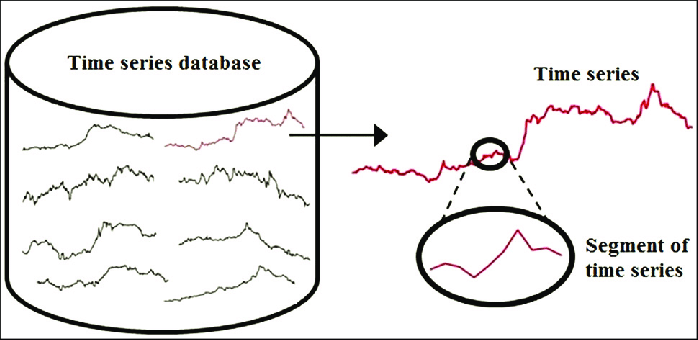
\includegraphics[scale=0.25]{./images/TSDB.png}
\caption{Schema of a time series database}
\end{figure}
\end{frame}

%%%%%%%%%%%%%%%%%%%%

\begin{frame}
\frametitle{Time series Database}
Common characteristics of TSDB include:
\begin{itemize}
\item Time series data is always collected over a specified time period.
\item Data from workloads is new and written as inserts, rather than updated to replace the data that already exists.
\item When data is written, it is automatically assigned to the most recent time interval.
\end{itemize}
\end{frame}

%%%%%%%%%%%%%%%%%%%%

\begin{frame}
\frametitle{Popular databases}
Examples of time series database options include InfluxDB, KairosDB, Prometheus and ClickHouse. These examples are open source, meaning anyone can access and edit the original source code.

Other popular TSDBs include:

\begin{itemize}
\item TimescaleDB,
\item OpenTSDB and
\item Graphite.
\end{itemize}
Times series databases are usually an extension of PostgreSQL databases, and they share similar features.
\end{frame}

%%%%%%%%%%%%%%%%%%%%

\section{What is Prometheus?}

\begin{frame}
\frametitle{Prometheus}

\begin{figure}
\centering

\includegraphics[height=60px]{./images/example-image.png}
\end{figure}

\textbf{Prometheus} is a system monitoring and alerting system. It was opensourced by SoundCloud in 2012 and is the second project both to join and to graduate within Cloud Native Computing Foundation after Kubernetes. Prometheus stores all metrics data as time series, i.e metrics information is stored along with the timestamp at which it was recorded, optional key-value pairs called as labels can also be stored along with metrics.
\end{frame}

%%%%%%%%%%%%%%%%%%%%

\begin{frame}
\begin{center}
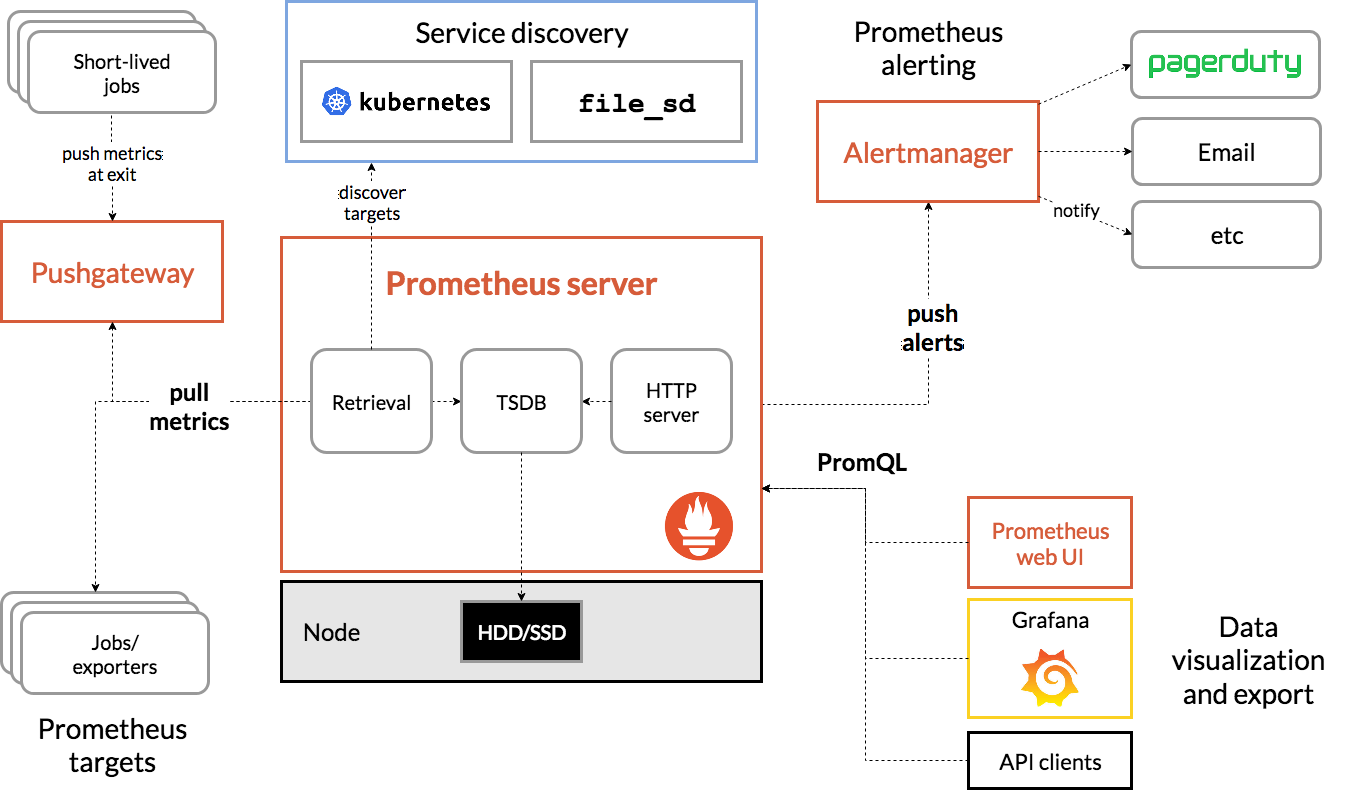
\includegraphics[height=150px]{./images/architecture.png}
\end{center}
\end{frame}

%%%%%%%%%%%%%%%%%%%%

\begin{frame}
\frametitle{Type of metrics in Prometheus}
\begin{enumerate}
\item \textbf{Counter} \\
Counter is a metric value which can only increase or reset i.e the value cannot reduce than the previous value. It can be used for metrics like number of requests, no of errors etc.
\item \textbf{Gauge} \\
Gauge is a number which can either go up or down. It can be used for metrics like number of pods in a cluster, number of events in an queue etc. 
\item \textbf{Histogram} \\
Histogram can be used for any calculated value which is counted based on bucket values. Bucket boundaries can be configured by the developer.
\item \textbf{Summary} \\
Summaries also measure events and are an alternative to histograms.
\end{enumerate}
\end{frame}

%%%%%%%%%%%%%%%%%%%%

\begin{frame}
\frametitle{Difference between histogram and summary}
\begin{itemize}
\item Summaries are cheaper than histograms.
\item Summaries lose more data than histograms.
\item They are calculated on the application level hence aggregation of metrics from multiple instances of the same process is not possible.
\item They are used when the buckets of a metric is not known beforehand, but it is highly recommended to use histograms over summaries whenever possible.
\end{itemize}
\end{frame}

%%%%%%%%%%%%%%%%%%%%

\section{What is Grafana?}

\begin{frame}

\begin{figure}
\centering

\includegraphics[height=60px]{./images/Grafana_logo.svg.png}
\end{figure}

Grafana is an open source interactive data-visualization platform, developed by Grafana Labs, which allows users to see their data via charts and graphs that are unified into one dashboard (or multiple dashboards!) for easier interpretation and understanding.

\end{frame}

%%%%%%%%%%%%%%%%%%%%

\subsection{Grafana Dashboard}
\begin{frame}
\frametitle{Grafana Dashboard}

Key features
\begin{itemize}

\item Panels: visualize your data any way you want using histograms, graphs, geomaps, heatmaps, etc.
\item Plugins: Render your data in real time on a user-friendly API via panel plugins that hook into existing data sources—no data migration required. You can also create data source plugins, retrieving metrics from any custom API.
\item Alerts: One user interface lets you create, consolidate, and control all your alerts.
\item Transformations: Rename, summarize, combine, and perform calculations across data sources and queries.
Annotations: Use rich events from different data sources to annotate graphs.
\item Panel Editor: A consistent user interface for configuring and customizing your panels.
\end{itemize}
\end{frame}

\end{document}
